% sections/04_infrastructure.tex

\section{Infrastructure Evolution}

% --- Slide 1: The Pre-Big Data Crisis ---
\begin{frame}{The Context: Why now and not before?}
    Before 2004, "Big Data" was handled by massive, expensive vertical mainframes. 

    \begin{columns}
        \begin{column}{0.65\textwidth}
            \begin{itemize}
                \item \textbf{The "Single Giant" (Vertical):} 
                    Hitting the physical and financial ceiling of a single machine.
                \item \textbf{The "Army of Ants" (Horizontal):} 
                    Linking 1,000 "commodity" PCs to act as one.
            \end{itemize}
            \vfill
            \begin{alertblock}{Economic Necessity}
                In the 90s, RAM was \textbf{>\$50/MB}. We switched because scaling vertically became \textbf{bankrupting}.
            \end{alertblock}
        \end{column}
        
        \begin{column}{0.35\textwidth}
            \centering
            % --- TikZ Floppy (Scaled 1.6x) ---
            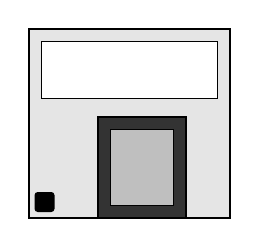
\begin{tikzpicture}[scale=0.8] 
                \draw[thick, fill=gray!20] (0,0) rectangle (3.2, 3.0);
                \draw[fill=white] (0.2, 1.9) rectangle (3.0, 2.8);
                \draw[thick, fill=black!80] (1.1, 0) rectangle (2.5, 1.6);
                \draw[fill=gray!50] (1.3, 0.2) rectangle (2.3, 1.4);
                \draw[rounded corners=1pt, fill=black] (0.1, 0.1) rectangle (0.4, 0.4);
            \end{tikzpicture}
        \end{column}
    \end{columns}
\end{frame}

% --- Slide 2: Google's Contributions ---
\begin{frame}{Google's Contributions (2004)}
    \begin{columns}
        \begin{column}{0.2\textwidth}
            \centering
            % --- TikZ Light Bulb (Scaled 1.6x) ---
            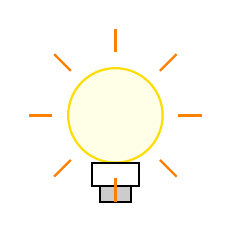
\begin{tikzpicture}[scale=1.0] 
                \draw[yellow!80!orange, thick, fill=yellow!10] (0,0) circle (0.6);
                \draw[thick] (-0.3,-0.6) rectangle (0.3,-0.9);
                \draw[thick, fill=gray!40] (-0.2,-0.9) rectangle (0.2,-1.1);
                \foreach \a in {0,45,...,315} \draw[orange, thick] (\a:0.8) -- (\a:1.1);
            \end{tikzpicture}
        \end{column}
        \begin{column}{0.8\textwidth}
            The \textit{"MapReduce"} paper by Dean \& Ghemawat:
            \begin{itemize}
                \item \textbf{Abstraction:} Simplified distributed math into Map/Reduce.
                \item \textbf{Fault Tolerance:} Hardware failure is now a software problem.
                \item \textbf{Data Locality:} "Move the computation, not the data."
            \end{itemize}
        \end{column}
    \end{columns}
    
    \vfill
    \begin{alertblock}{The Catalyst for Innovation}
        By sharing this blueprint, Google allowed the community to build \textbf{Apache Hadoop}, moving beyond the "Single Giant" era.
    \end{alertblock}
\end{frame}

% --- Slide 3: Evolution of Speed (Hadoop vs Spark) ---
\begin{frame}{From the "Basement" to the "Desk"}
    \begin{columns}
        \begin{column}{0.75\textwidth}
            \begin{itemize}
                \item \textbf{Hadoop Era (2006):} Relied on Disk. Like a librarian walking to the \textbf{basement} for every book.
                \item \textbf{Spark Era (2014):} Uses RAM (RDDs). The librarian keeps everything on the \textbf{desk}.
            \end{itemize}
        \end{column}
        \begin{column}{0.25\textwidth}
            \centering
            % --- TikZ Level Up (Scaled 1.6x) ---
            
\begin{tikzpicture}[scale=0.65] 
                \draw[cyan, line width=4pt, ->] (0,0) -- (0,3);
                \node[cyan, font=\small\bfseries, align=center] at (0,3.6) {LEVEL\\UP};
            \end{tikzpicture}
        \end{column}
    \end{columns}

    \vfill
    \begin{table}
        \centering
        \footnotesize
        \begin{tabular}{|l|c|c|}
            \hline
            \textbf{Feature} & \textbf{Hadoop (Disk)} & \textbf{Spark (RAM)} \\ \hline
            Processing Speed & 1x & \textbf{100x Faster} \\ \hline
            Data Access & Sequential & \textbf{Instant (RDD)} \\ \hline
        \end{tabular}
    \end{table}
\end{frame}

% --- Slide 4: Spark Architecture \& The New Bottleneck ---
\begin{frame}{Spark Architecture \& The New Bottleneck}
    \begin{itemize}
        \item \textbf{The Setup:} Database partitioned across the cluster's RAM.
        \item \textbf{The Pattern:} Candidates ($C_k$) are broadcast to every worker.
    \end{itemize}

    \vfill
    \begin{alertblock}{The CPU Wall}
        Data is now in RAM, so the disk is no longer the problem. The new bottleneck is the \textbf{CPU} searching millions of candidates per second.
    \end{alertblock}

    \vfill
    \begin{center}
        \footnotesize \itshape Coming up: A deep dive into the \textbf{Data Structures} that will solve this bottleneck...
    \end{center}
\end{frame}
